\chapter{\textit{File} Teks Soal-Soal Permainan Calcudoku untuk Pengujian}
\label{chap:soalsoal}

Lampiran ini berisi \textit{file} teks dari soal-soal permainan Calcudoku yang dipakai dalam pengujian ini. Soal-soal ini diambil dari sumber-sumber berikut:

\begin{enumerate}
\item \url{https://iota.math.msu.edu/k12-outreach/kenken-puzzles/}
\item \url{http://thinkmath.edc.org/resource/kenken-puzzles}
\end{enumerate}

\twocolumn[\section{\textit{File} Teks Soal-Soal Permainan Calcudoku dengan \textit{Grid} Berukuran 4 $\times$ 4} \label{sec:soalsoal4x4}]

\lstinputlisting[caption=4x4\_1.txt]{PuzzleFiles/4x4_1.txt}
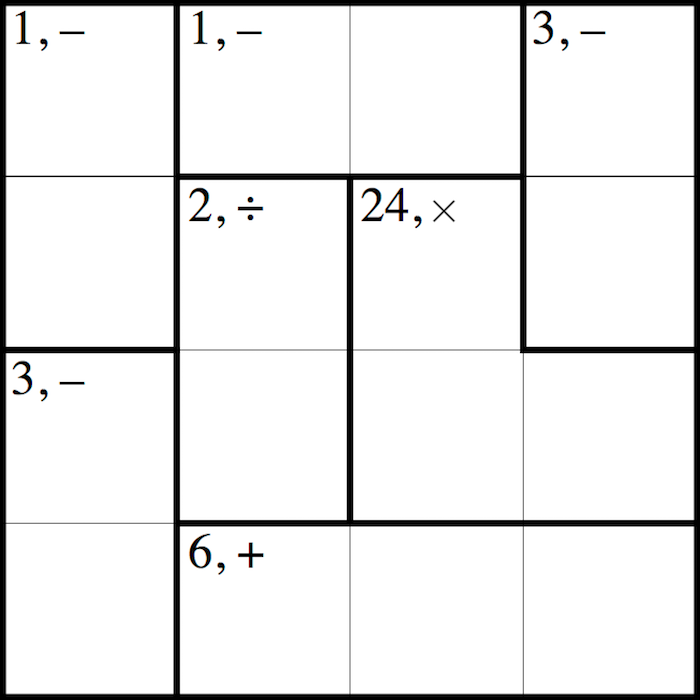
\includegraphics[scale=1]{Gambar/Lampiran/4x4_1.png}
\lstinputlisting[caption=4x4\_2.txt]{PuzzleFiles/4x4_2.txt}
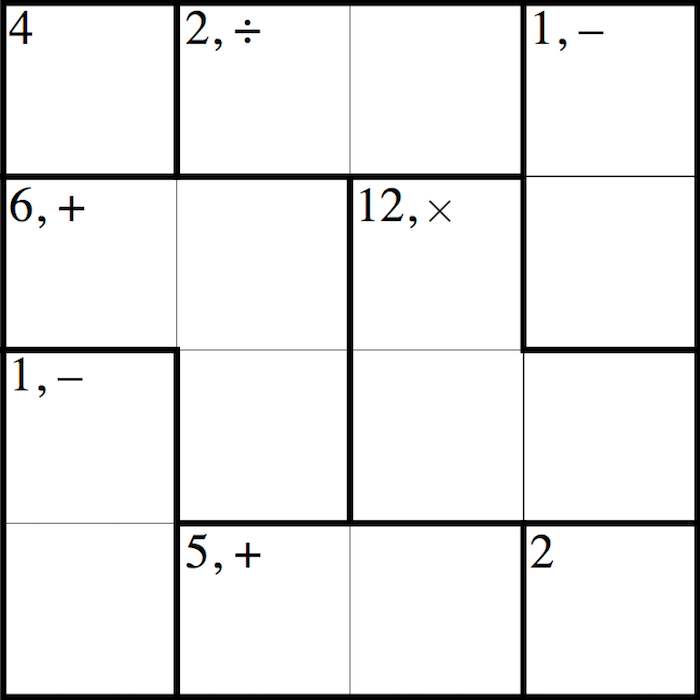
\includegraphics[scale=1]{Gambar/Lampiran/4x4_2.png}
\lstinputlisting[caption=4x4\_3.txt]{PuzzleFiles/4x4_3.txt}
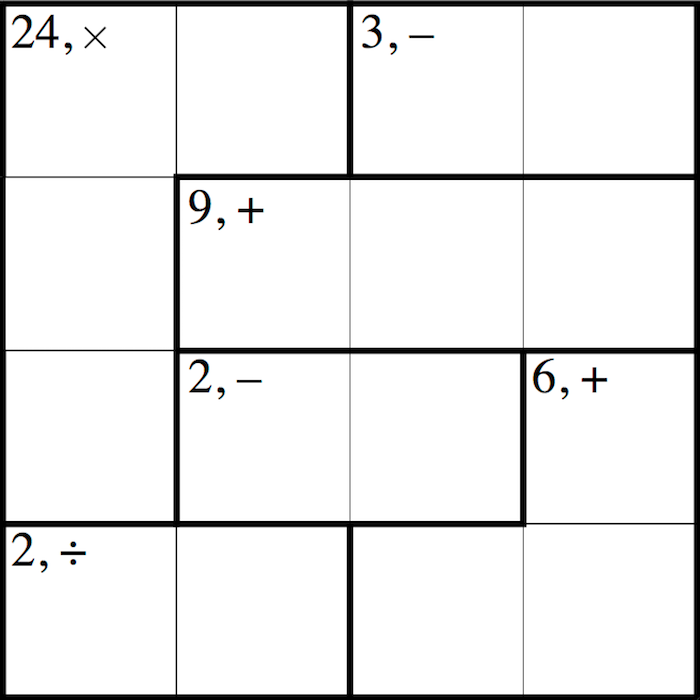
\includegraphics[scale=1]{Gambar/Lampiran/4x4_3.png}
\lstinputlisting[caption=4x4\_4.txt]{PuzzleFiles/4x4_4.txt}
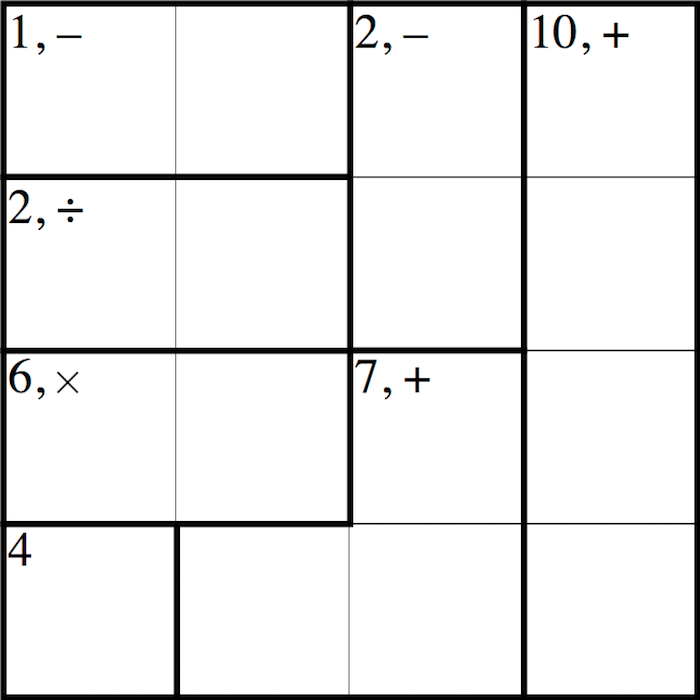
\includegraphics[scale=1]{Gambar/Lampiran/4x4_4.png}
\lstinputlisting[caption=4x4\_5.txt]{PuzzleFiles/4x4_5.txt}
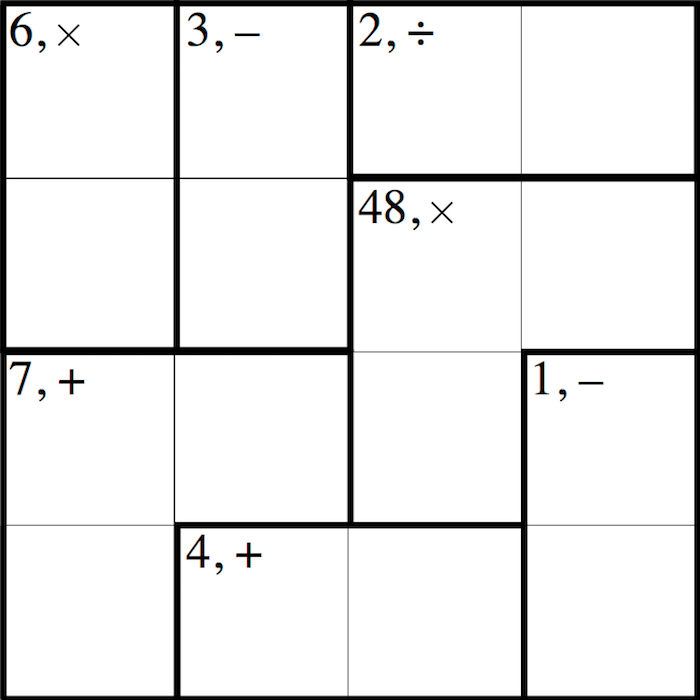
\includegraphics[scale=1]{Gambar/Lampiran/4x4_5.png}
\lstinputlisting[caption=4x4\_6.txt]{PuzzleFiles/4x4_6.txt}
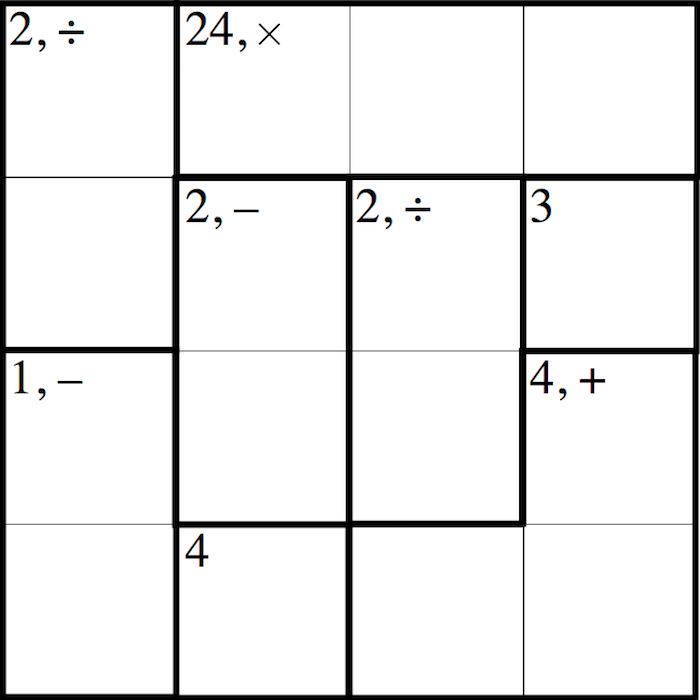
\includegraphics[scale=1]{Gambar/Lampiran/4x4_6.png}
\lstinputlisting[caption=4x4\_7.txt]{PuzzleFiles/4x4_7.txt}
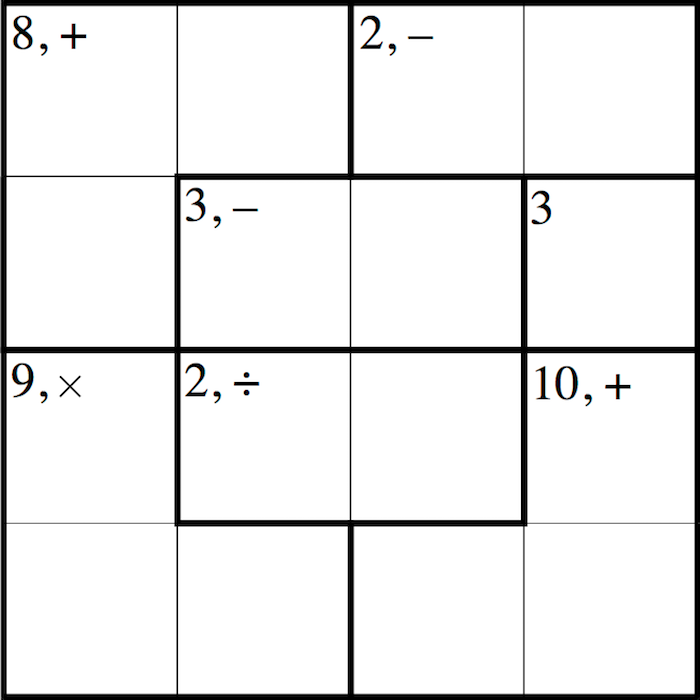
\includegraphics[scale=1]{Gambar/Lampiran/4x4_7.png}
\lstinputlisting[caption=4x4\_8.txt]{PuzzleFiles/4x4_8.txt}
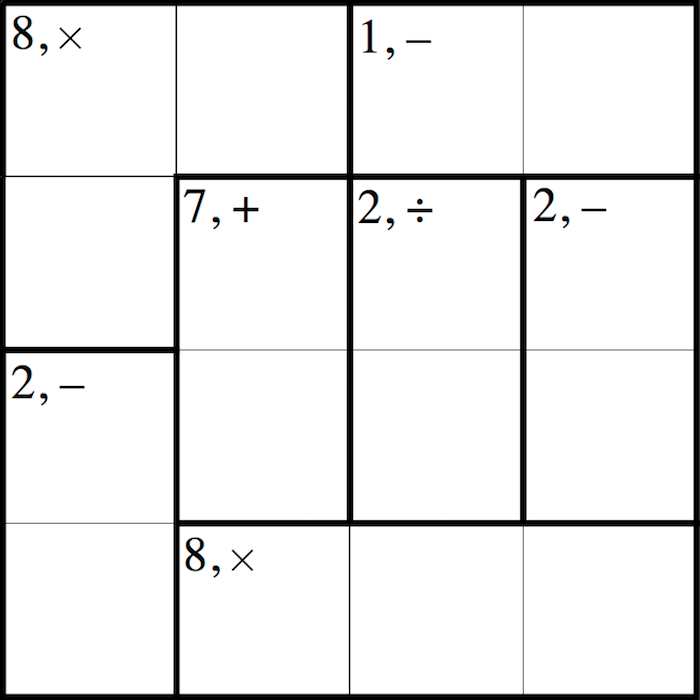
\includegraphics[scale=1]{Gambar/Lampiran/4x4_8.png}
\lstinputlisting[caption=4x4\_9.txt]{PuzzleFiles/4x4_9.txt}
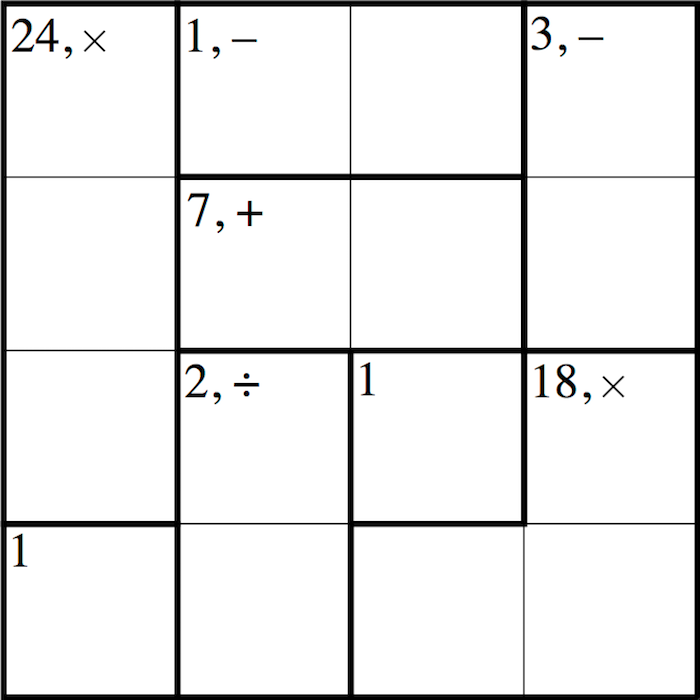
\includegraphics[scale=1]{Gambar/Lampiran/4x4_9.png}
\lstinputlisting[caption=4x4\_10.txt]{PuzzleFiles/4x4_10.txt}
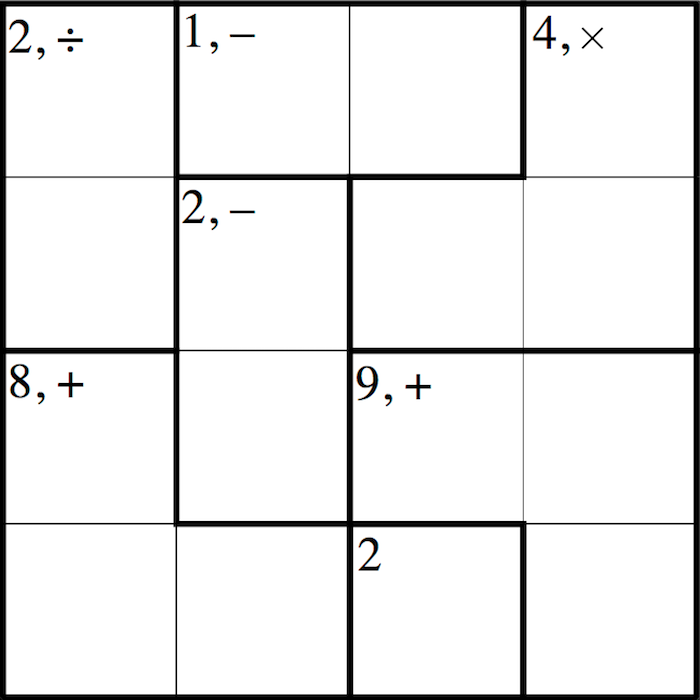
\includegraphics[scale=1]{Gambar/Lampiran/4x4_10.png}
\lstinputlisting[caption=4x4\_11.txt]{PuzzleFiles/4x4_11.txt}
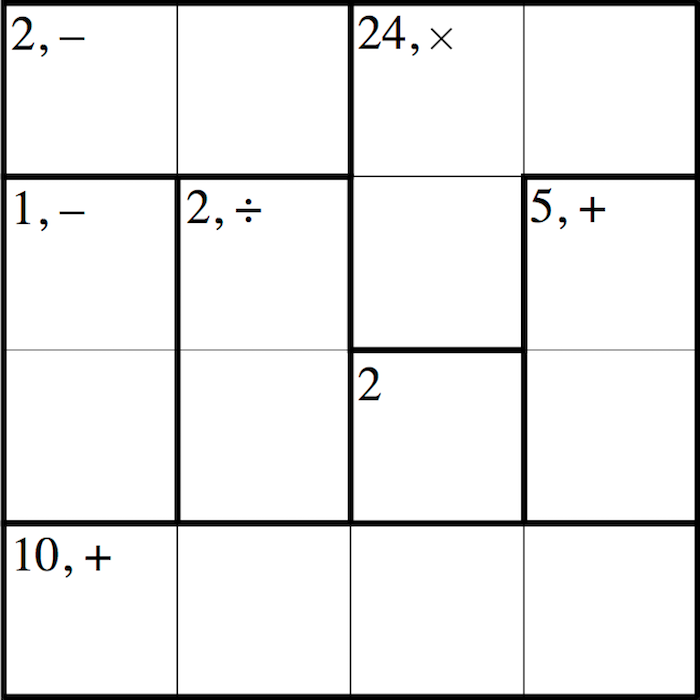
\includegraphics[scale=1]{Gambar/Lampiran/4x4_11.png}
\lstinputlisting[caption=4x4\_12.txt]{PuzzleFiles/4x4_12.txt}
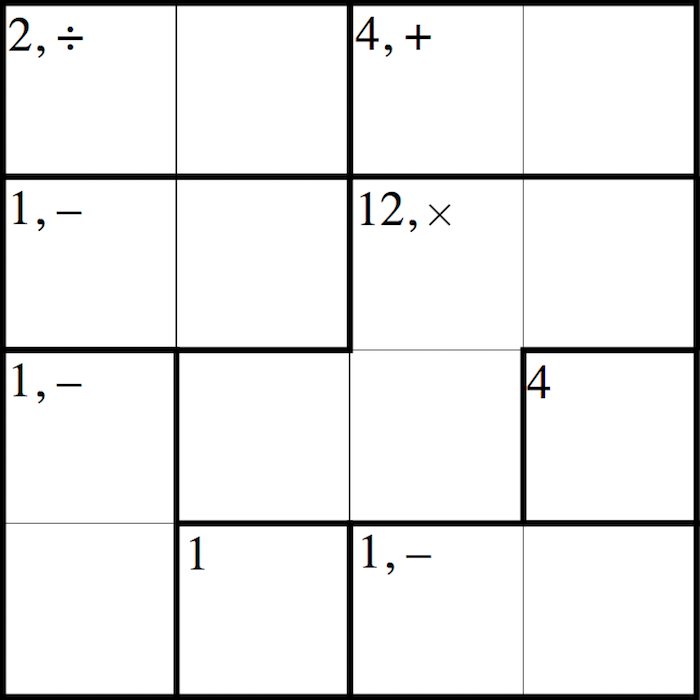
\includegraphics[scale=1]{Gambar/Lampiran/4x4_12.png}
\lstinputlisting[caption=4x4\_13.txt]{PuzzleFiles/4x4_13.txt}
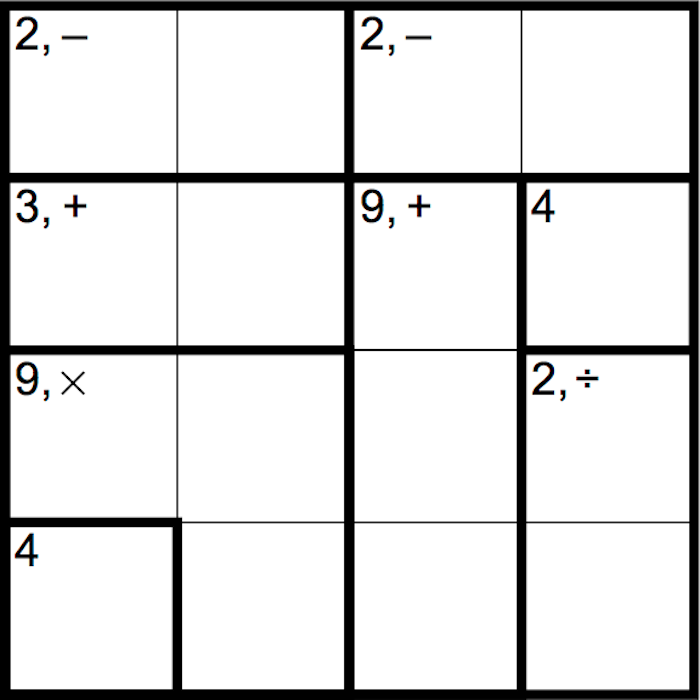
\includegraphics[scale=1]{Gambar/Lampiran/4x4_13.png}
\lstinputlisting[caption=4x4\_14.txt]{PuzzleFiles/4x4_14.txt}
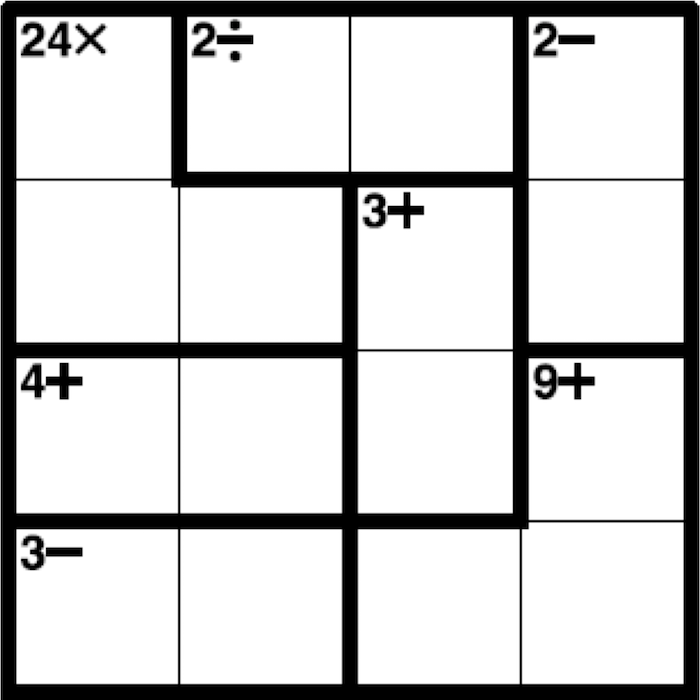
\includegraphics[scale=1]{Gambar/Lampiran/4x4_14.png}
\lstinputlisting[caption=4x4\_15.txt]{PuzzleFiles/4x4_15.txt}
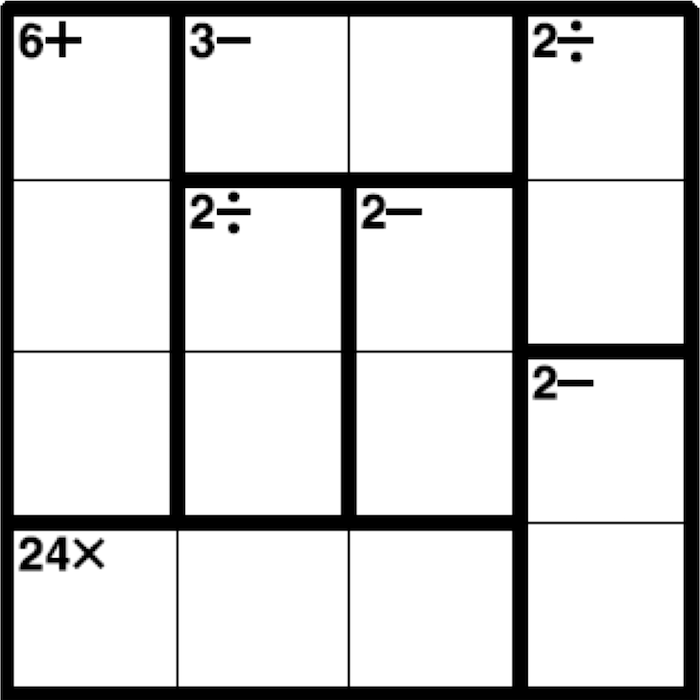
\includegraphics[scale=1]{Gambar/Lampiran/4x4_15.png}
\lstinputlisting[caption=4x4\_16.txt]{PuzzleFiles/4x4_16.txt}
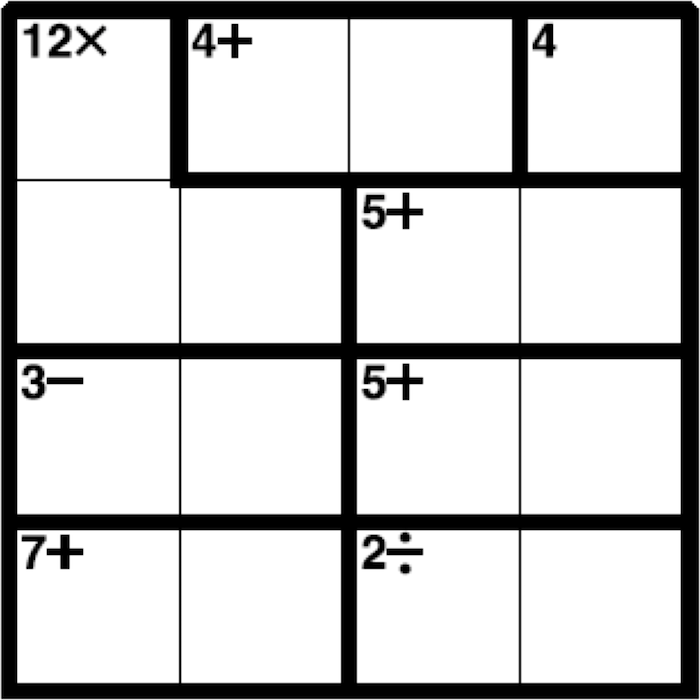
\includegraphics[scale=1]{Gambar/Lampiran/4x4_16.png}
\lstinputlisting[caption=4x4\_17.txt]{PuzzleFiles/4x4_17.txt}
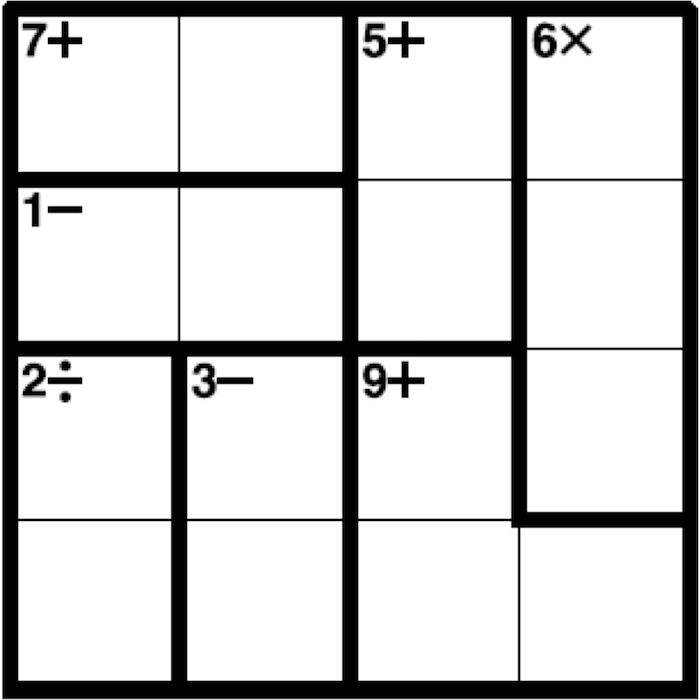
\includegraphics[scale=1]{Gambar/Lampiran/4x4_17.png}
\lstinputlisting[caption=4x4\_18.txt]{PuzzleFiles/4x4_18.txt}
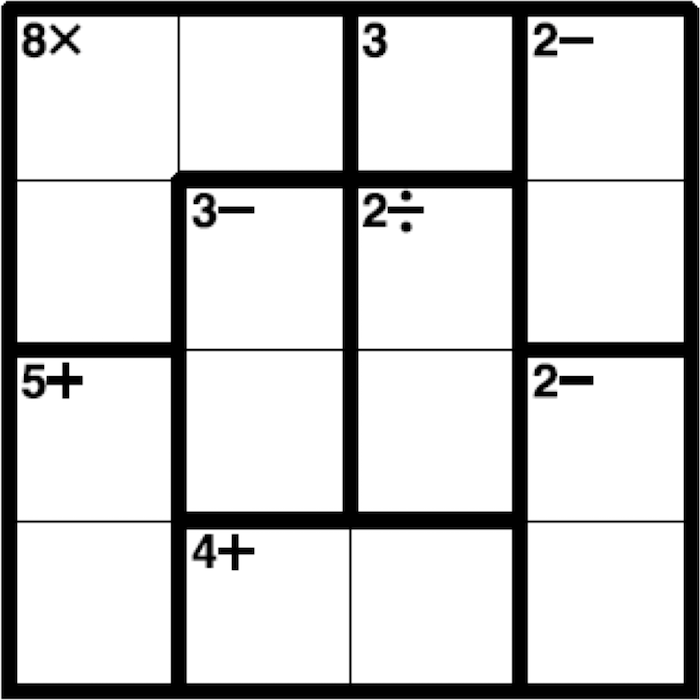
\includegraphics[scale=1]{Gambar/Lampiran/4x4_18.png}
\lstinputlisting[caption=4x4\_19.txt]{PuzzleFiles/4x4_19.txt}
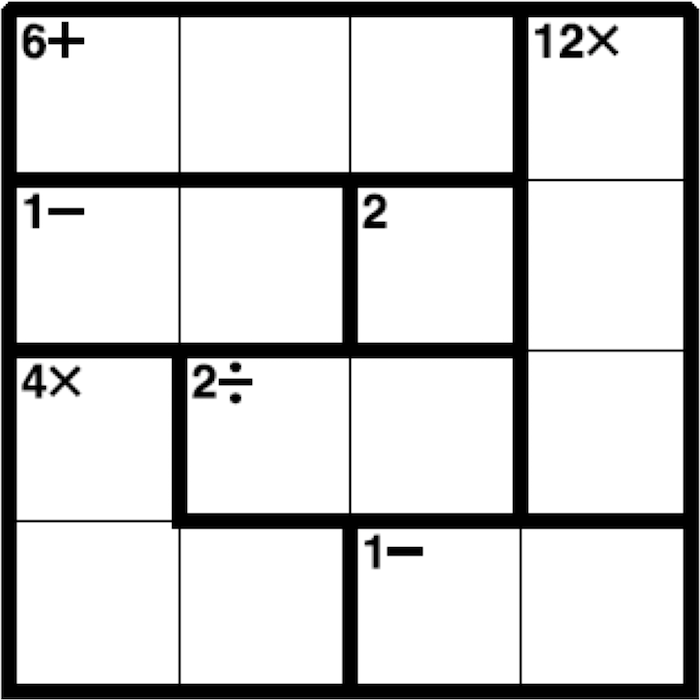
\includegraphics[scale=1]{Gambar/Lampiran/4x4_19.png}
\lstinputlisting[caption=4x4\_20.txt]{PuzzleFiles/4x4_20.txt}
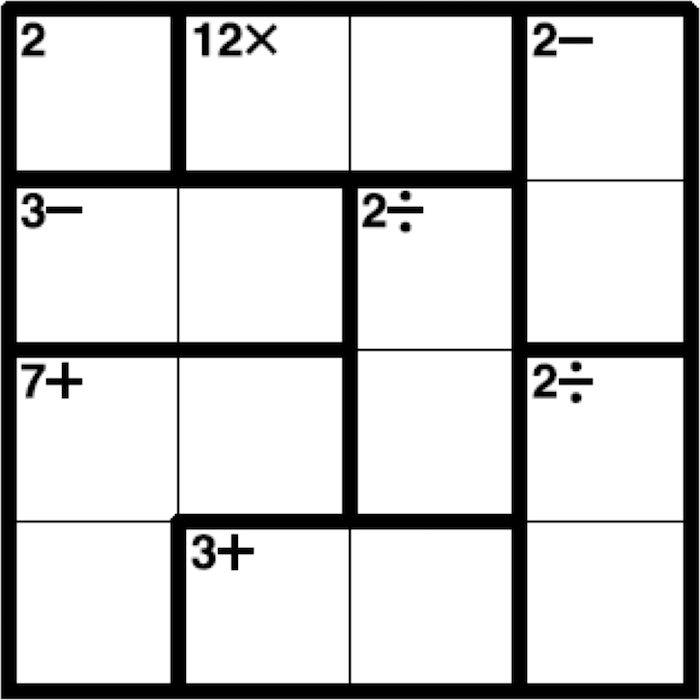
\includegraphics[scale=1]{Gambar/Lampiran/4x4_20.png}
\lstinputlisting[caption=4x4\_21.txt]{PuzzleFiles/4x4_21.txt}
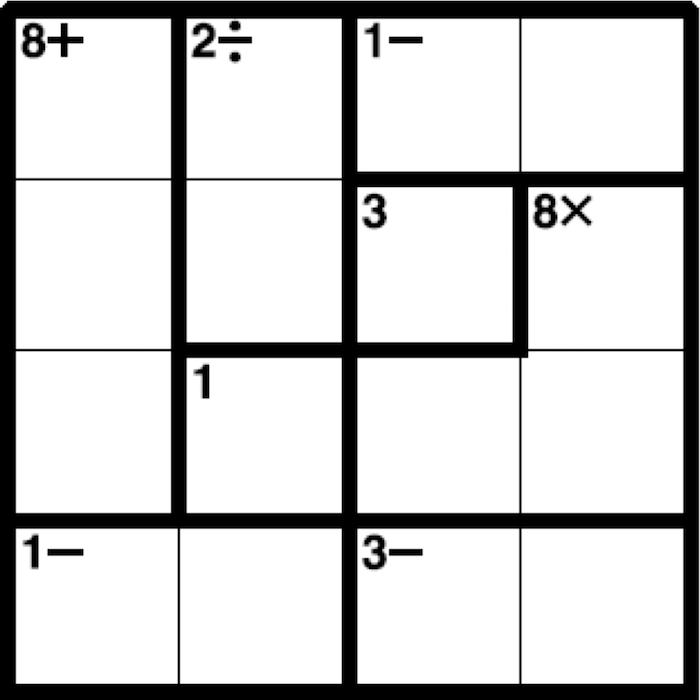
\includegraphics[scale=1]{Gambar/Lampiran/4x4_21.png}
\lstinputlisting[caption=4x4\_22.txt]{PuzzleFiles/4x4_22.txt}
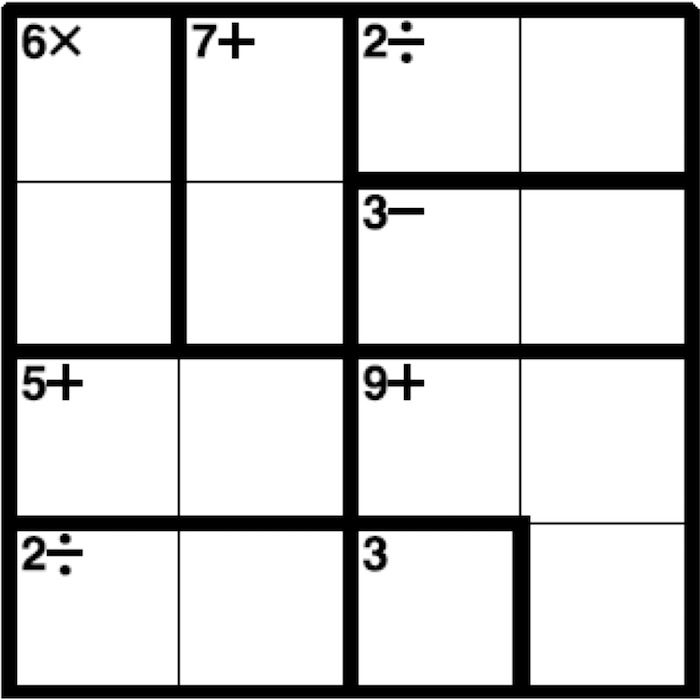
\includegraphics[scale=1]{Gambar/Lampiran/4x4_22.png}
\lstinputlisting[caption=4x4\_23.txt]{PuzzleFiles/4x4_23.txt}
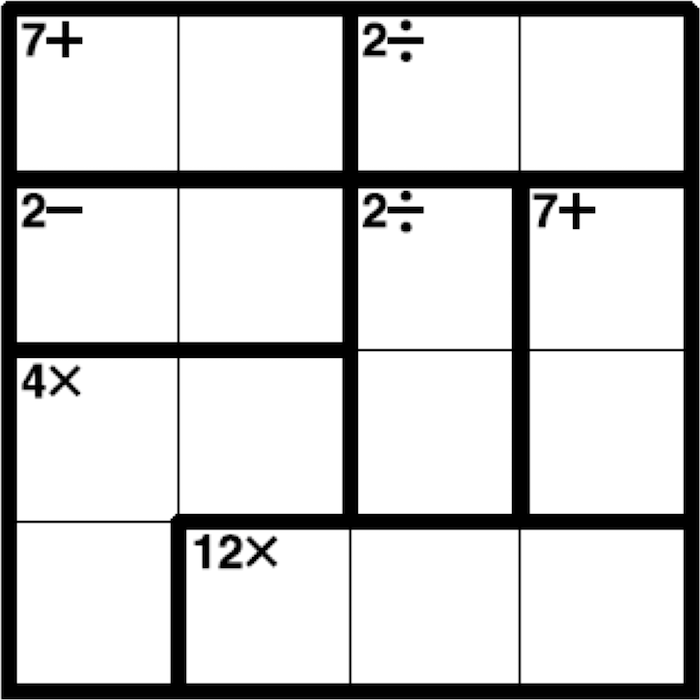
\includegraphics[scale=1]{Gambar/Lampiran/4x4_23.png}
\lstinputlisting[caption=4x4\_24.txt]{PuzzleFiles/4x4_24.txt}
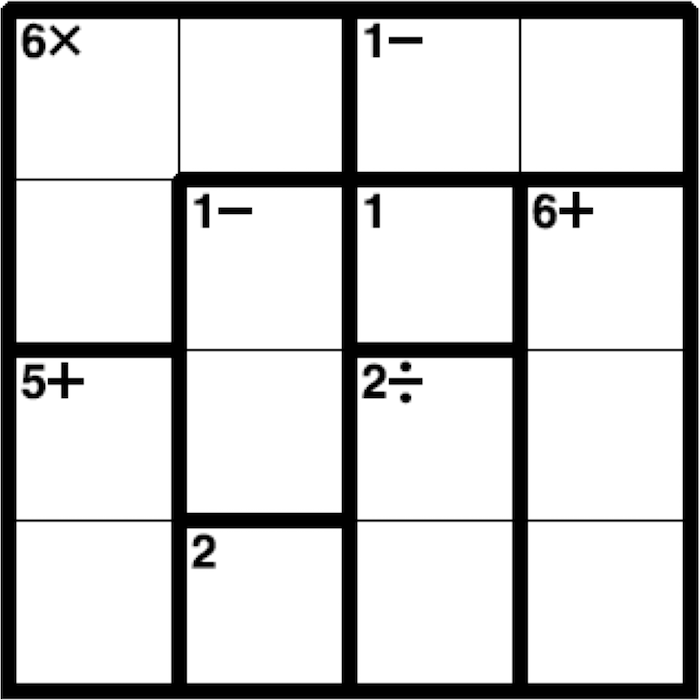
\includegraphics[scale=1]{Gambar/Lampiran/4x4_24.png}
\lstinputlisting[caption=4x4\_25.txt]{PuzzleFiles/4x4_25.txt}
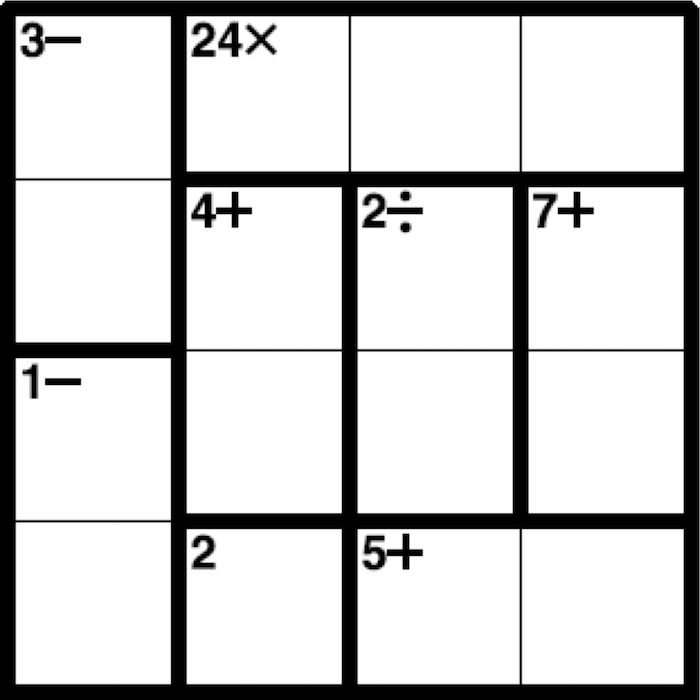
\includegraphics[scale=1]{Gambar/Lampiran/4x4_25.png}
\lstinputlisting[caption=4x4\_26.txt]{PuzzleFiles/4x4_26.txt}
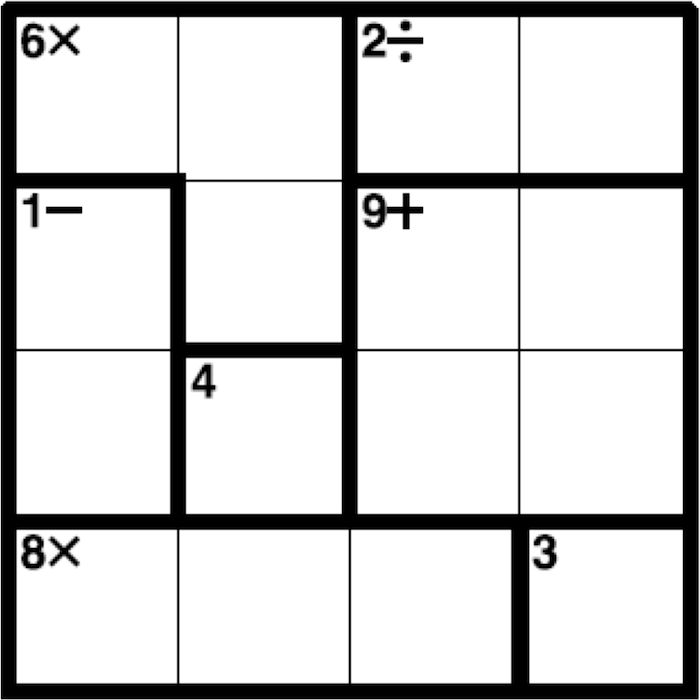
\includegraphics[scale=1]{Gambar/Lampiran/4x4_26.png}
\lstinputlisting[caption=4x4\_27.txt]{PuzzleFiles/4x4_27.txt}
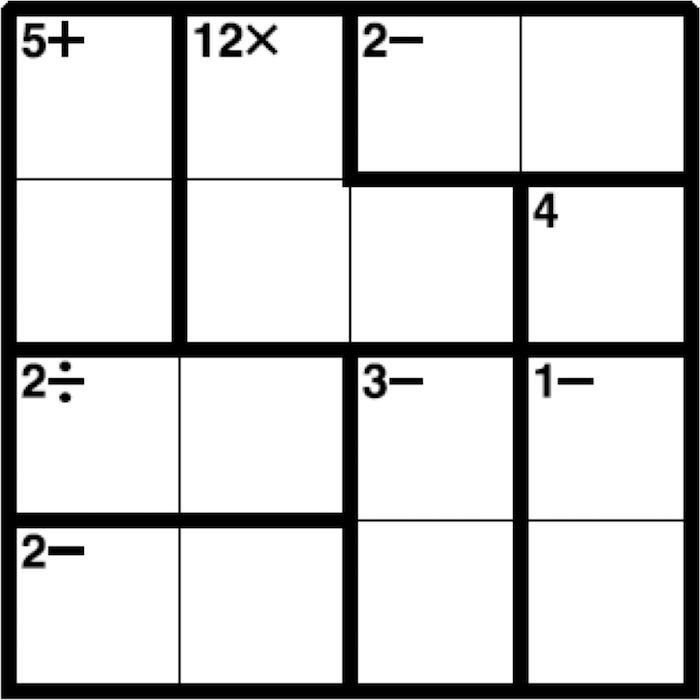
\includegraphics[scale=1]{Gambar/Lampiran/4x4_27.png}
\lstinputlisting[caption=4x4\_28.txt]{PuzzleFiles/4x4_28.txt}
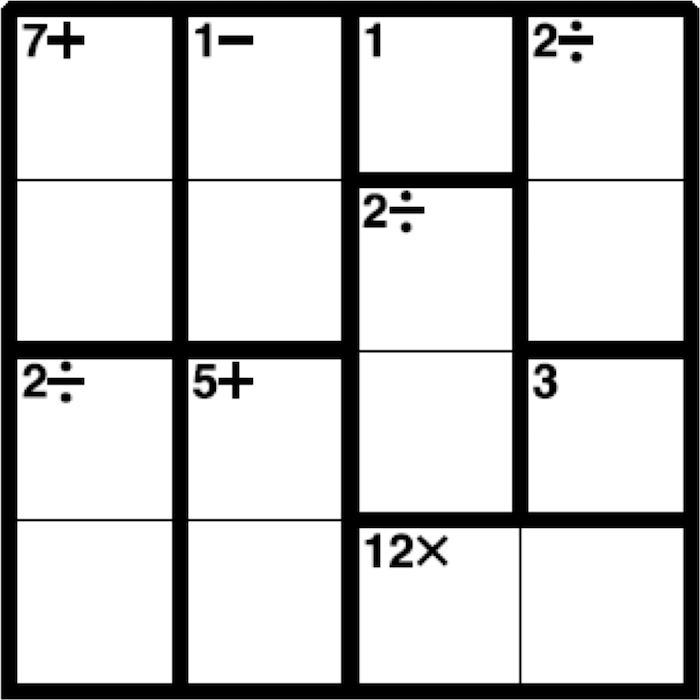
\includegraphics[scale=1]{Gambar/Lampiran/4x4_28.png}
\lstinputlisting[caption=4x4\_29.txt]{PuzzleFiles/4x4_29.txt}
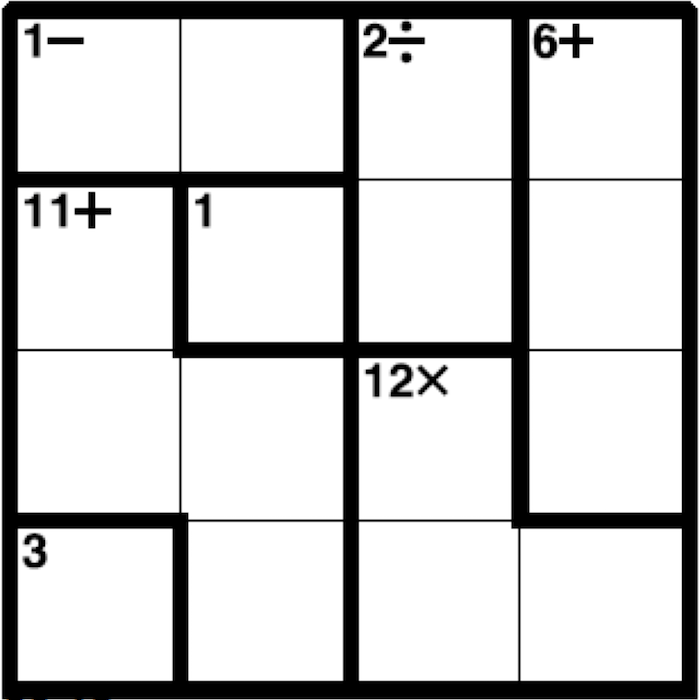
\includegraphics[scale=1]{Gambar/Lampiran/4x4_29.png}
\lstinputlisting[caption=4x4\_30.txt]{PuzzleFiles/4x4_30.txt}
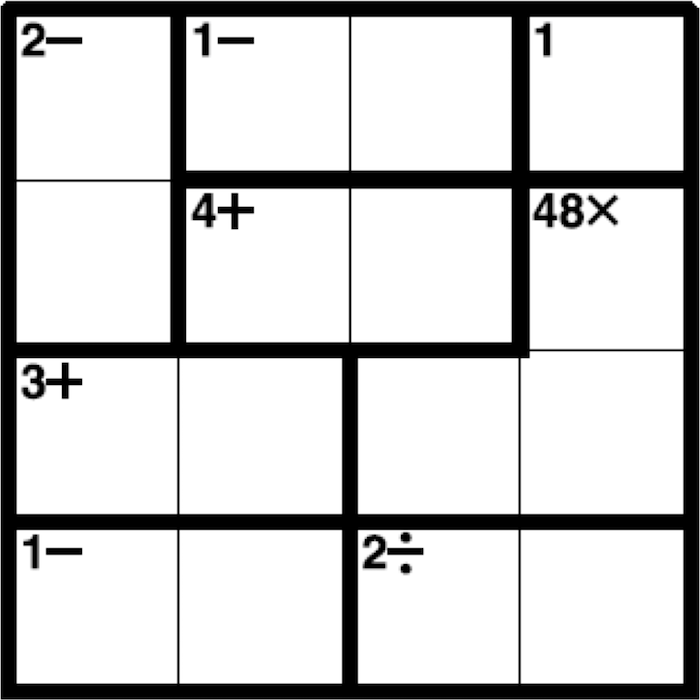
\includegraphics[scale=1]{Gambar/Lampiran/4x4_30.png}
\lstinputlisting[caption=4x4\_31.txt]{PuzzleFiles/4x4_31.txt}
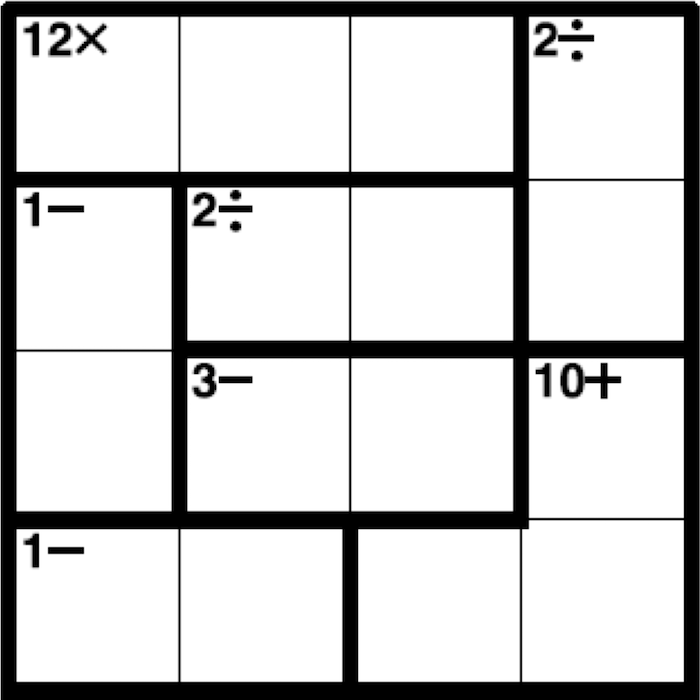
\includegraphics[scale=1]{Gambar/Lampiran/4x4_31.png}
\lstinputlisting[caption=4x4\_32.txt]{PuzzleFiles/4x4_32.txt}
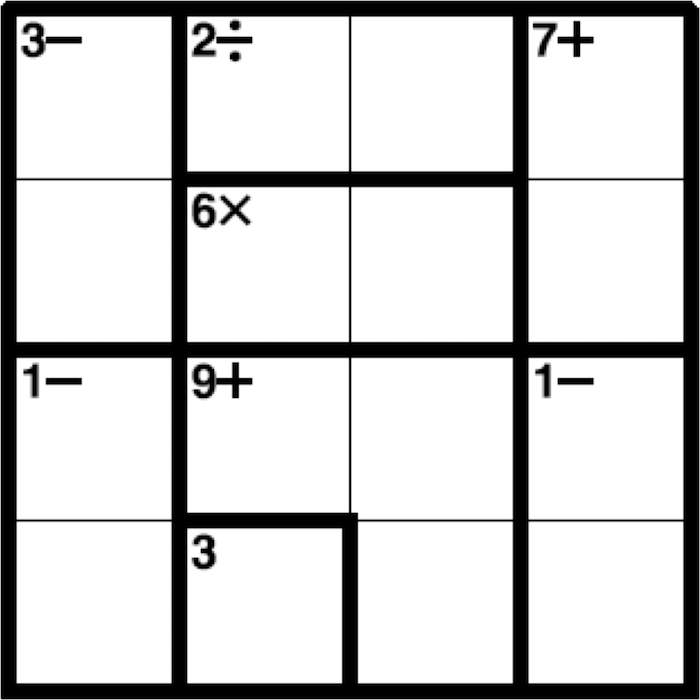
\includegraphics[scale=1]{Gambar/Lampiran/4x4_32.png}
\lstinputlisting[caption=4x4\_33.txt]{PuzzleFiles/4x4_33.txt}
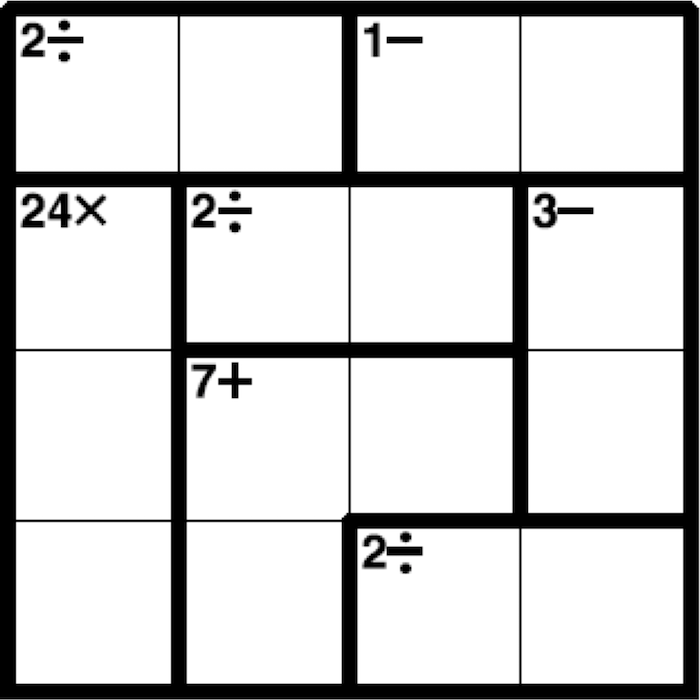
\includegraphics[scale=1]{Gambar/Lampiran/4x4_33.png}
\lstinputlisting[caption=4x4\_34.txt]{PuzzleFiles/4x4_34.txt}
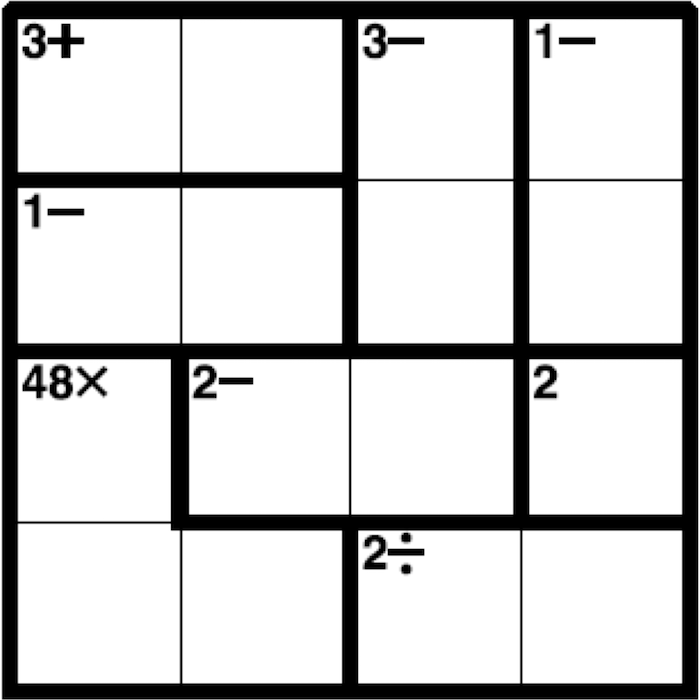
\includegraphics[scale=1]{Gambar/Lampiran/4x4_34.png}
\lstinputlisting[caption=4x4\_35.txt]{PuzzleFiles/4x4_35.txt}
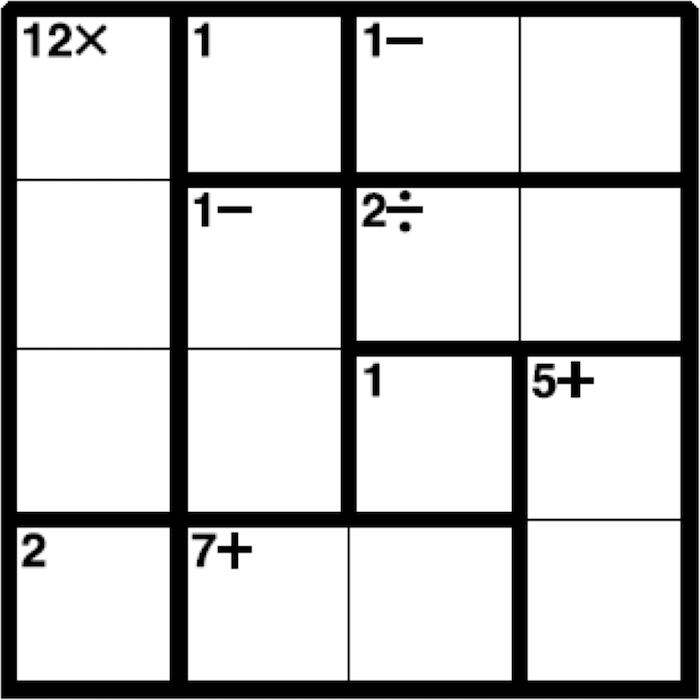
\includegraphics[scale=1]{Gambar/Lampiran/4x4_35.png}
\lstinputlisting[caption=4x4\_36.txt]{PuzzleFiles/4x4_36.txt}
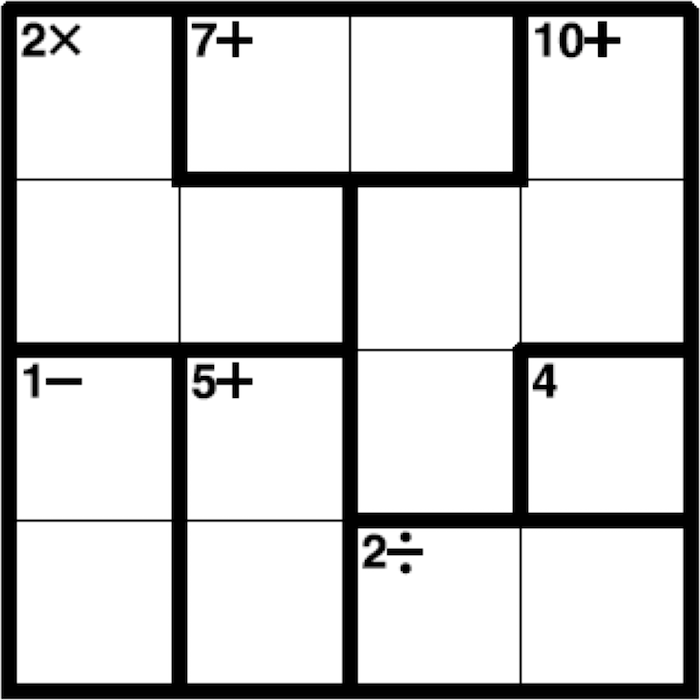
\includegraphics[scale=1]{Gambar/Lampiran/4x4_36.png}
\lstinputlisting[caption=4x4\_37.txt]{PuzzleFiles/4x4_37.txt}
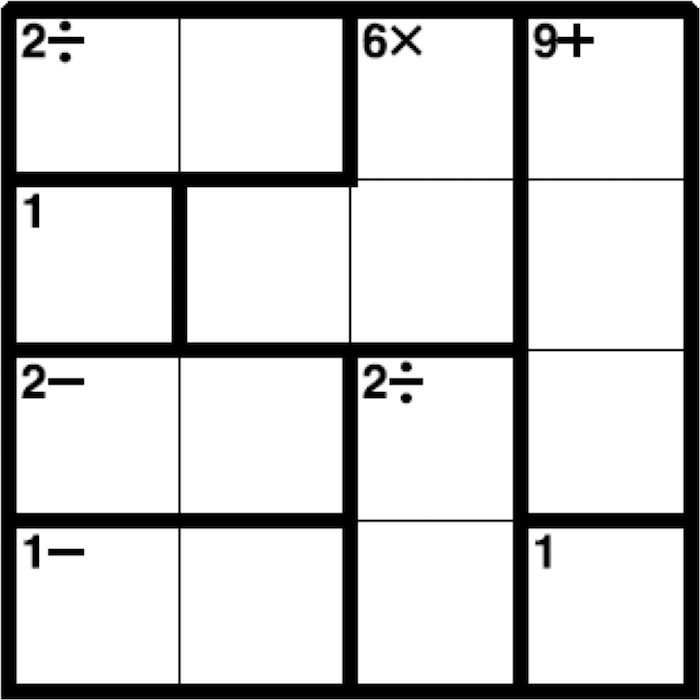
\includegraphics[scale=1]{Gambar/Lampiran/4x4_37.png}
\lstinputlisting[caption=4x4\_38.txt]{PuzzleFiles/4x4_38.txt}
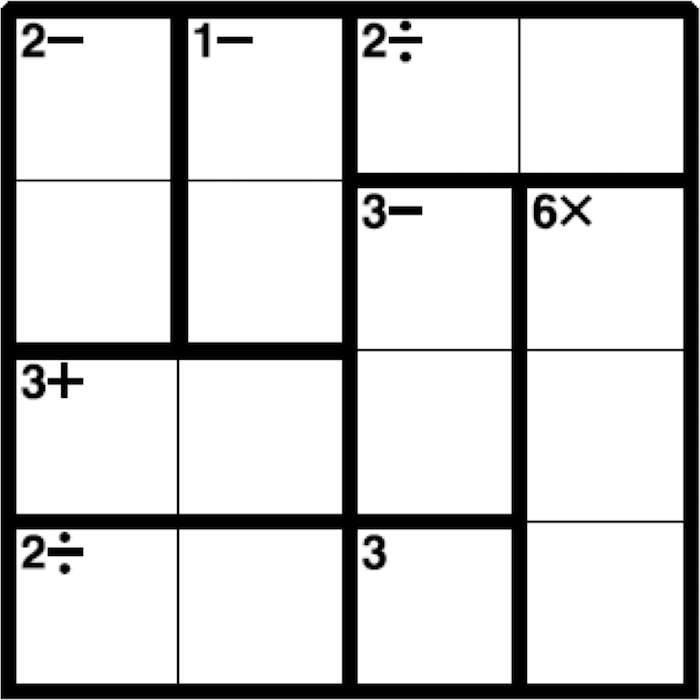
\includegraphics[scale=1]{Gambar/Lampiran/4x4_38.png}
\lstinputlisting[caption=4x4\_39.txt]{PuzzleFiles/4x4_39.txt}
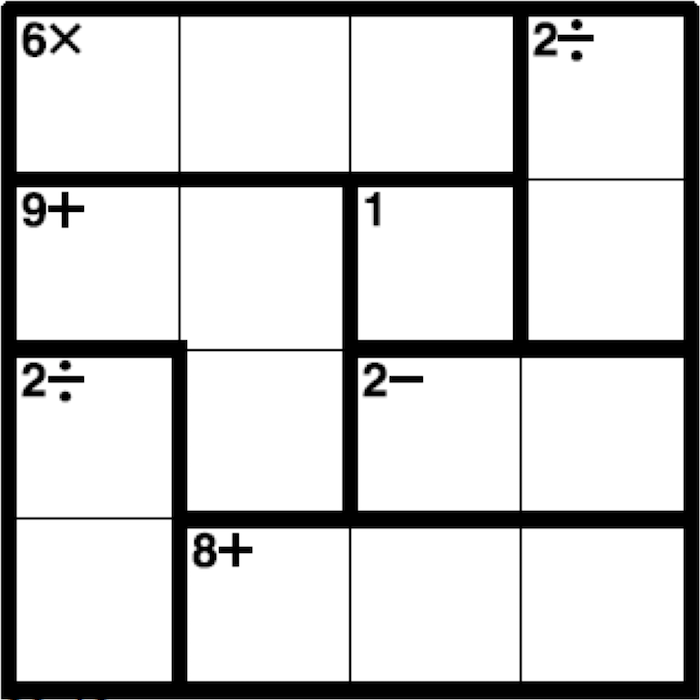
\includegraphics[scale=1]{Gambar/Lampiran/4x4_39.png}

\onecolumn

\twocolumn[\section{\textit{File} Teks Soal-Soal Permainan Calcudoku dengan \textit{Grid} Berukuran 5 $\times$ 5} \label{sec:soalsoal5x5}]

\lstinputlisting[caption=5x5\_1.txt]{PuzzleFiles/5x5_1.txt}
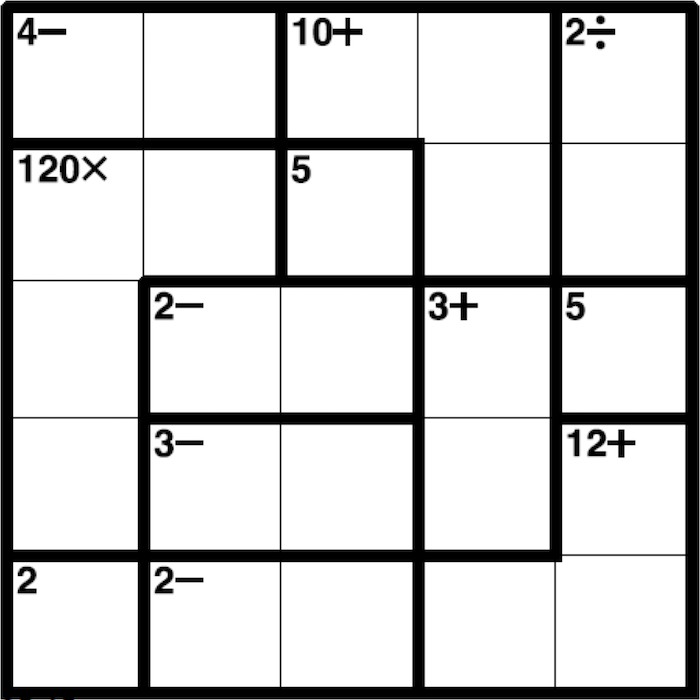
\includegraphics[scale=1]{Gambar/Lampiran/5x5_1.png}
\lstinputlisting[caption=5x5\_2.txt]{PuzzleFiles/5x5_2.txt}
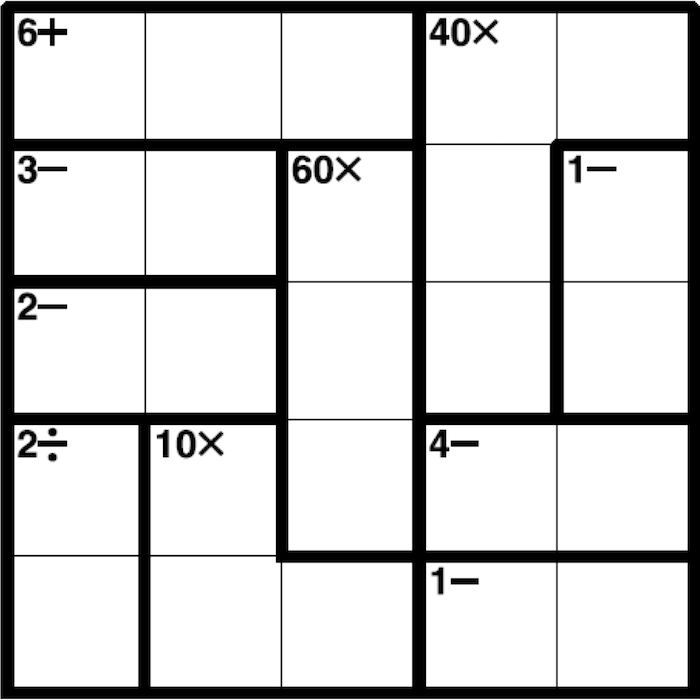
\includegraphics[scale=1]{Gambar/Lampiran/5x5_2.png}
\lstinputlisting[caption=5x5\_3.txt]{PuzzleFiles/5x5_3.txt}
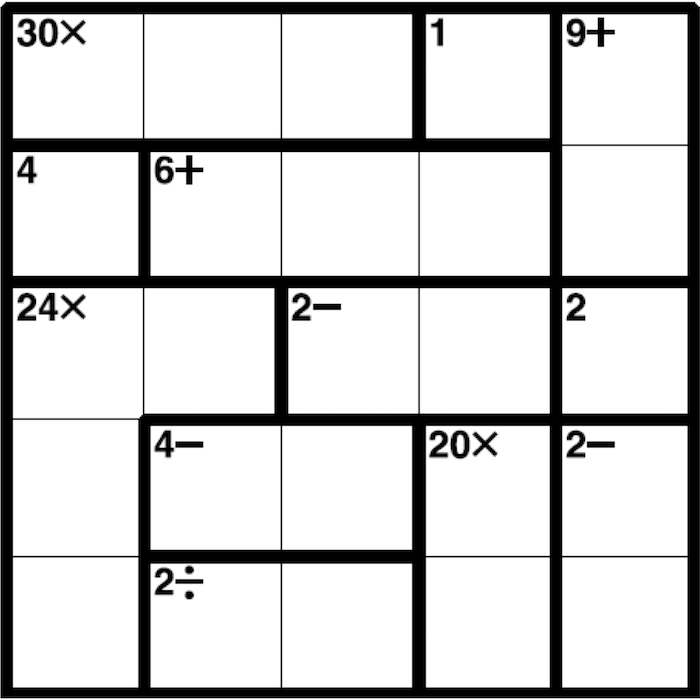
\includegraphics[scale=1]{Gambar/Lampiran/5x5_3.png}
\lstinputlisting[caption=5x5\_4.txt]{PuzzleFiles/5x5_4.txt}
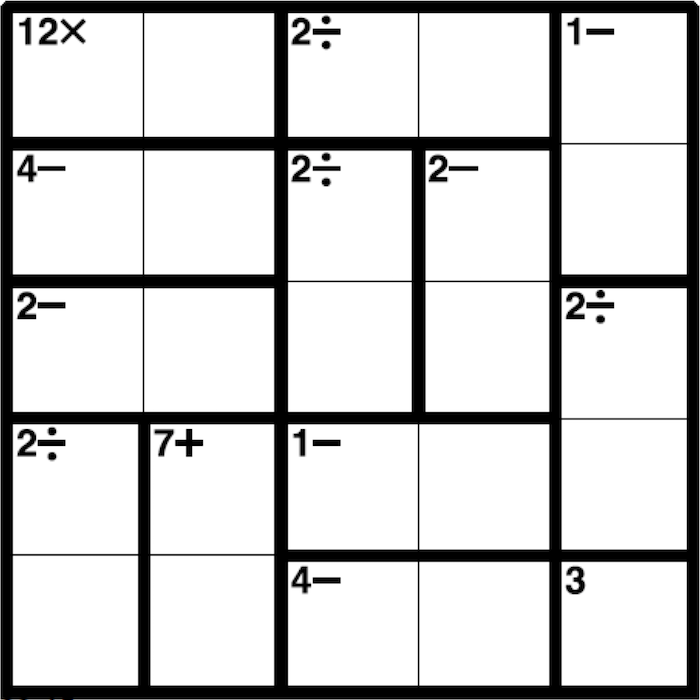
\includegraphics[scale=1]{Gambar/Lampiran/5x5_4.png}
\lstinputlisting[caption=5x5\_5.txt]{PuzzleFiles/5x5_5.txt}
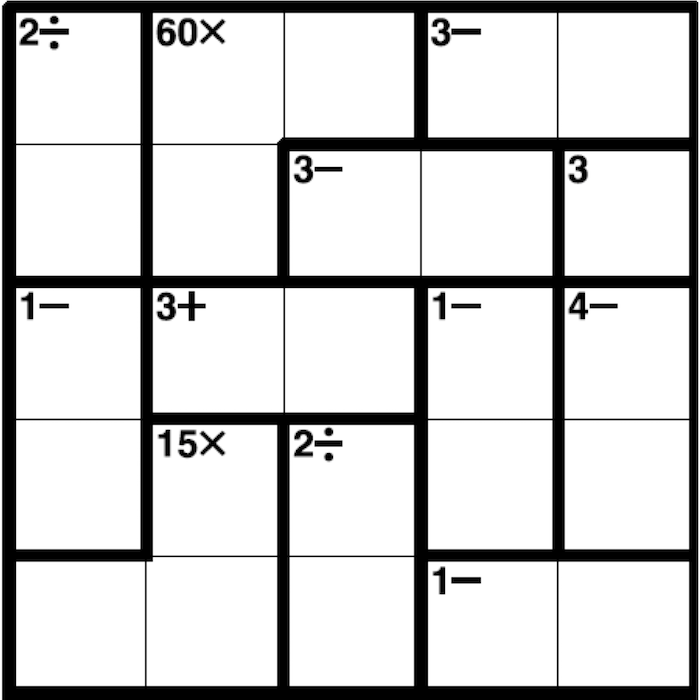
\includegraphics[scale=1]{Gambar/Lampiran/5x5_5.png}
\lstinputlisting[caption=5x5\_6.txt]{PuzzleFiles/5x5_6.txt}
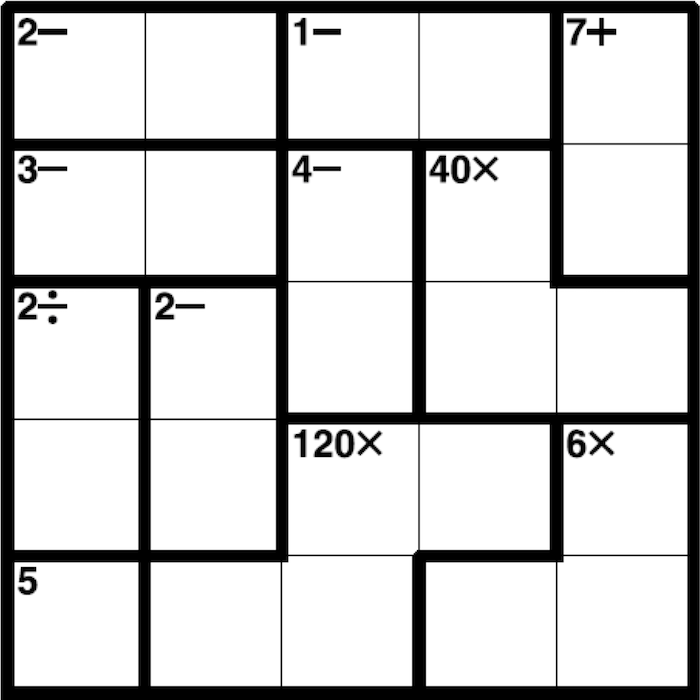
\includegraphics[scale=1]{Gambar/Lampiran/5x5_6.png}
\lstinputlisting[caption=5x5\_7.txt]{PuzzleFiles/5x5_7.txt}
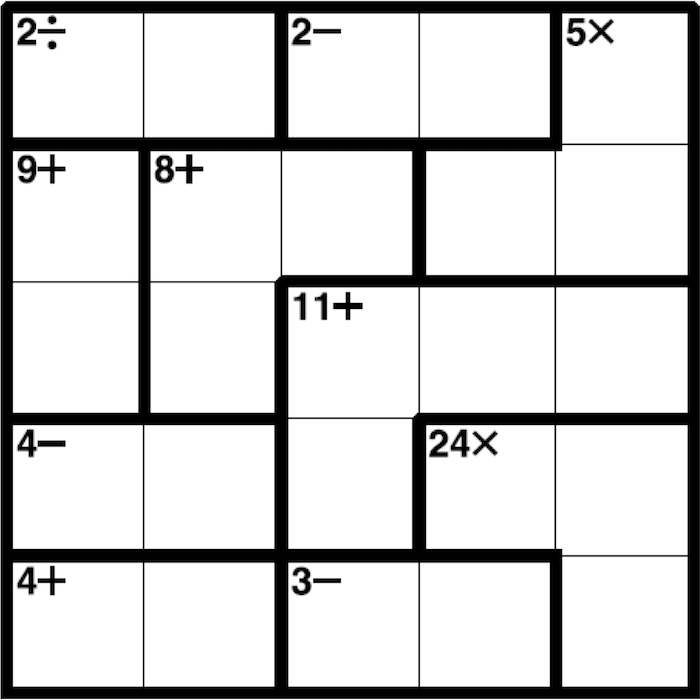
\includegraphics[scale=1]{Gambar/Lampiran/5x5_7.png}
\lstinputlisting[caption=5x5\_8.txt]{PuzzleFiles/5x5_8.txt}
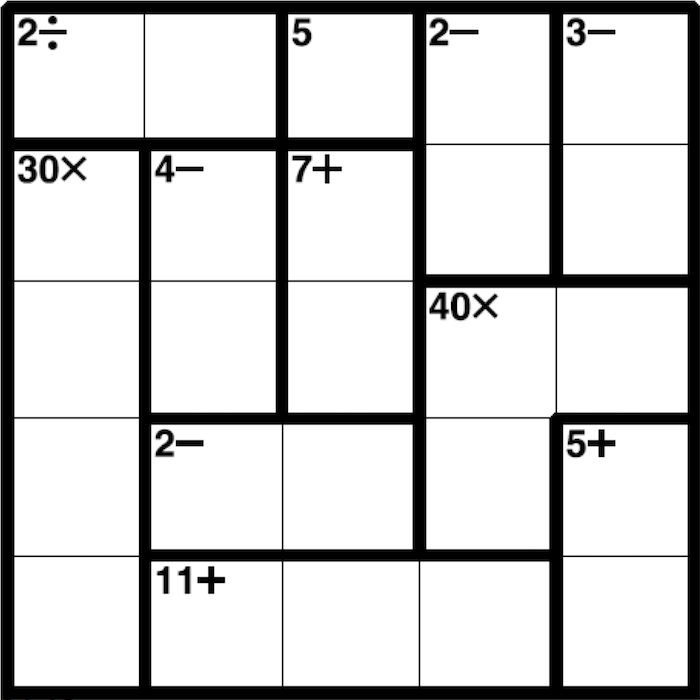
\includegraphics[scale=1]{Gambar/Lampiran/5x5_8.png}
\lstinputlisting[caption=5x5\_9.txt]{PuzzleFiles/5x5_9.txt}
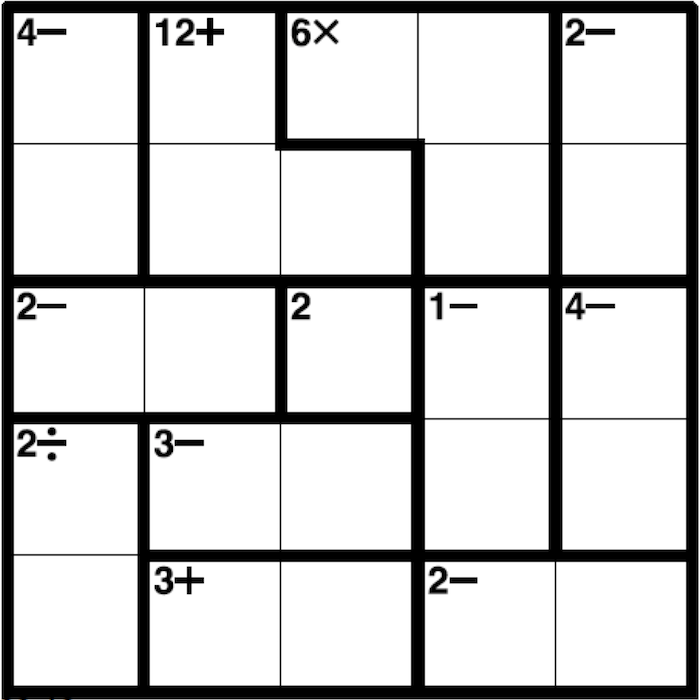
\includegraphics[scale=1]{Gambar/Lampiran/5x5_9.png}
\lstinputlisting[caption=5x5\_10.txt]{PuzzleFiles/5x5_10.txt}
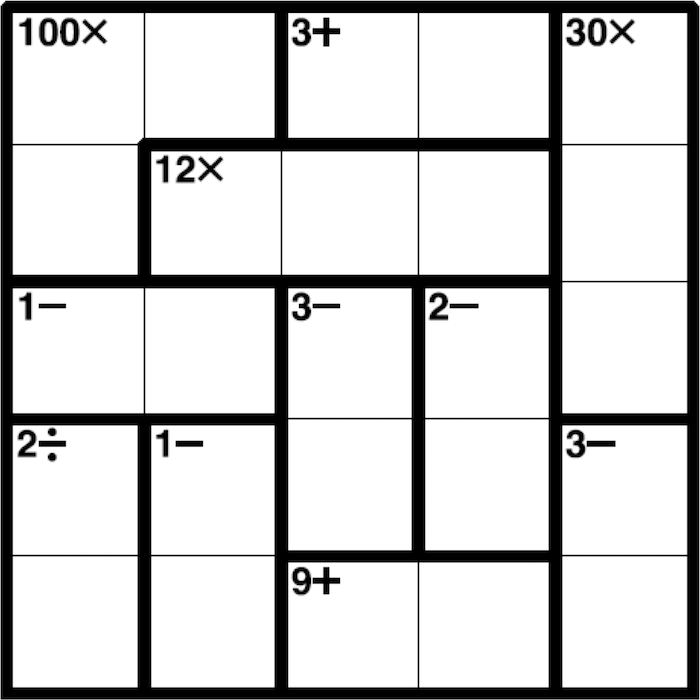
\includegraphics[scale=1]{Gambar/Lampiran/5x5_10.png}
\lstinputlisting[caption=5x5\_11.txt]{PuzzleFiles/5x5_11.txt}
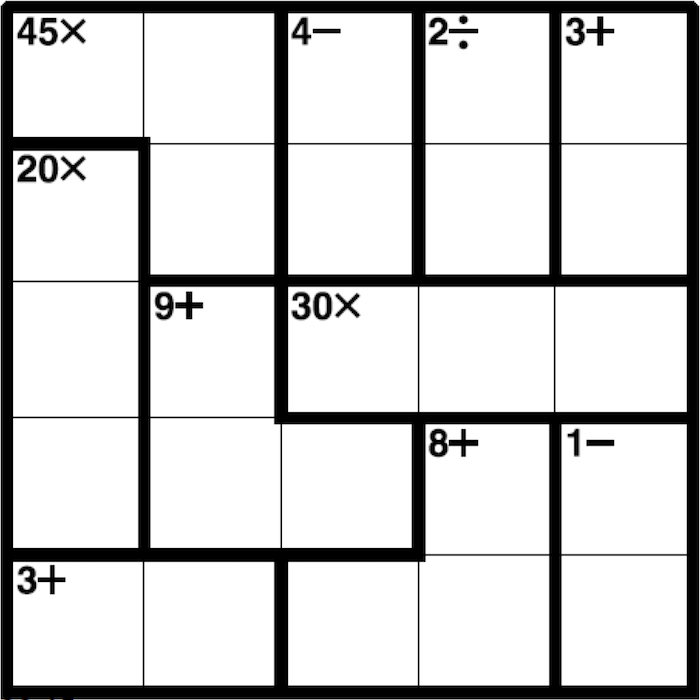
\includegraphics[scale=1]{Gambar/Lampiran/5x5_11.png}
\lstinputlisting[caption=5x5\_12.txt]{PuzzleFiles/5x5_12.txt}
\includegraphics[scale=1]{Gambar/Lampiran/5x5_12.png}
\lstinputlisting[caption=5x5\_13.txt]{PuzzleFiles/5x5_13.txt}
\includegraphics[scale=1]{Gambar/Lampiran/5x5_13.png}
\lstinputlisting[caption=5x5\_14.txt]{PuzzleFiles/5x5_14.txt}
\includegraphics[scale=1]{Gambar/Lampiran/5x5_14.png}
\lstinputlisting[caption=5x5\_15.txt]{PuzzleFiles/5x5_15.txt}
\includegraphics[scale=1]{Gambar/Lampiran/5x5_15.png}
\lstinputlisting[caption=5x5\_16.txt]{PuzzleFiles/5x5_16.txt}
\includegraphics[scale=1]{Gambar/Lampiran/5x5_16.png}
\lstinputlisting[caption=5x5\_17.txt]{PuzzleFiles/5x5_17.txt}
\includegraphics[scale=1]{Gambar/Lampiran/5x5_17.png}
\lstinputlisting[caption=5x5\_18.txt]{PuzzleFiles/5x5_18.txt}
\includegraphics[scale=1]{Gambar/Lampiran/5x5_18.png}
\lstinputlisting[caption=5x5\_19.txt]{PuzzleFiles/5x5_19.txt}
\includegraphics[scale=1]{Gambar/Lampiran/5x5_19.png}
\lstinputlisting[caption=5x5\_20.txt]{PuzzleFiles/5x5_20.txt}
\includegraphics[scale=1]{Gambar/Lampiran/5x5_20.png}
\lstinputlisting[caption=5x5\_21.txt]{PuzzleFiles/5x5_21.txt}
\includegraphics[scale=1]{Gambar/Lampiran/5x5_21.png}
\lstinputlisting[caption=5x5\_22.txt]{PuzzleFiles/5x5_22.txt}
\includegraphics[scale=1]{Gambar/Lampiran/5x5_22.png}
\lstinputlisting[caption=5x5\_23.txt]{PuzzleFiles/5x5_23.txt}
\includegraphics[scale=1]{Gambar/Lampiran/5x5_23.png}
\lstinputlisting[caption=5x5\_24.txt]{PuzzleFiles/5x5_24.txt}
\includegraphics[scale=1]{Gambar/Lampiran/5x5_24.png}
\lstinputlisting[caption=5x5\_25.txt]{PuzzleFiles/5x5_25.txt}
\includegraphics[scale=1]{Gambar/Lampiran/5x5_25.png}
\lstinputlisting[caption=5x5\_26.txt]{PuzzleFiles/5x5_26.txt}
\includegraphics[scale=1]{Gambar/Lampiran/5x5_26.png}

\onecolumn

\twocolumn[\section{\textit{File} Teks Soal-Soal Permainan Calcudoku dengan \textit{Grid} Berukuran 6 $\times$ 6} \label{sec:soalsoal6x6}]

\lstinputlisting[caption=6x6\_1.txt]{PuzzleFiles/6x6_1.txt}
\includegraphics[scale=1]{Gambar/Lampiran/6x6_1.png}
\lstinputlisting[caption=6x6\_2.txt]{PuzzleFiles/6x6_2.txt}
\includegraphics[scale=1]{Gambar/Lampiran/6x6_2.png}
\lstinputlisting[caption=6x6\_3.txt]{PuzzleFiles/6x6_3.txt}
\includegraphics[scale=1]{Gambar/Lampiran/6x6_3.png}
\lstinputlisting[caption=6x6\_4.txt]{PuzzleFiles/6x6_4.txt}
\includegraphics[scale=1]{Gambar/Lampiran/6x6_4.png}
\lstinputlisting[caption=6x6\_5.txt]{PuzzleFiles/6x6_5.txt}
\includegraphics[scale=1]{Gambar/Lampiran/6x6_5.png}
\lstinputlisting[caption=6x6\_6.txt]{PuzzleFiles/6x6_6.txt}
\includegraphics[scale=1]{Gambar/Lampiran/6x6_6.png}
\lstinputlisting[caption=6x6\_7.txt]{PuzzleFiles/6x6_7.txt}
\includegraphics[scale=1]{Gambar/Lampiran/6x6_7.png}
\lstinputlisting[caption=6x6\_8.txt]{PuzzleFiles/6x6_8.txt}
\includegraphics[scale=1]{Gambar/Lampiran/6x6_8.png}
\lstinputlisting[caption=6x6\_9.txt]{PuzzleFiles/6x6_9.txt}
\includegraphics[scale=1]{Gambar/Lampiran/6x6_9.png}
\lstinputlisting[caption=6x6\_10.txt]{PuzzleFiles/6x6_10.txt}
\includegraphics[scale=1]{Gambar/Lampiran/6x6_10.png}
\lstinputlisting[caption=6x6\_11.txt]{PuzzleFiles/6x6_11.txt}
\includegraphics[scale=1]{Gambar/Lampiran/6x6_11.png}
\lstinputlisting[caption=6x6\_12.txt]{PuzzleFiles/6x6_12.txt}
\includegraphics[scale=1]{Gambar/Lampiran/6x6_12.png}
\lstinputlisting[caption=6x6\_13.txt]{PuzzleFiles/6x6_13.txt}
\includegraphics[scale=1]{Gambar/Lampiran/6x6_13.png}
\lstinputlisting[caption=6x6\_14.txt]{PuzzleFiles/6x6_14.txt}
\includegraphics[scale=1]{Gambar/Lampiran/6x6_14.png}
\lstinputlisting[caption=6x6\_15.txt]{PuzzleFiles/6x6_15.txt}
\includegraphics[scale=1]{Gambar/Lampiran/6x6_15.png}
\lstinputlisting[caption=6x6\_16.txt]{PuzzleFiles/6x6_16.txt}
\includegraphics[scale=1]{Gambar/Lampiran/6x6_16.png}
\lstinputlisting[caption=6x6\_17.txt]{PuzzleFiles/6x6_17.txt}
\includegraphics[scale=1]{Gambar/Lampiran/6x6_17.png}
\lstinputlisting[caption=6x6\_18.txt]{PuzzleFiles/6x6_18.txt}
\includegraphics[scale=1]{Gambar/Lampiran/6x6_18.png}
\lstinputlisting[caption=6x6\_19.txt]{PuzzleFiles/6x6_19.txt}
\includegraphics[scale=1]{Gambar/Lampiran/6x6_19.png}
\lstinputlisting[caption=6x6\_20.txt]{PuzzleFiles/6x6_20.txt}
\includegraphics[scale=1]{Gambar/Lampiran/6x6_20.png}
\lstinputlisting[caption=6x6\_21.txt]{PuzzleFiles/6x6_21.txt}
\includegraphics[scale=1]{Gambar/Lampiran/6x6_21.png}
\lstinputlisting[caption=6x6\_22.txt]{PuzzleFiles/6x6_22.txt}
\includegraphics[scale=1]{Gambar/Lampiran/6x6_22.png}
\lstinputlisting[caption=6x6\_23.txt]{PuzzleFiles/6x6_23.txt}
\includegraphics[scale=1]{Gambar/Lampiran/6x6_23.png}
\lstinputlisting[caption=6x6\_24.txt]{PuzzleFiles/6x6_24.txt}
\includegraphics[scale=1]{Gambar/Lampiran/6x6_24.png}
\lstinputlisting[caption=6x6\_25.txt]{PuzzleFiles/6x6_25.txt}
\includegraphics[scale=1]{Gambar/Lampiran/6x6_25.png}
\lstinputlisting[caption=6x6\_26.txt]{PuzzleFiles/6x6_26.txt}
\includegraphics[scale=1]{Gambar/Lampiran/6x6_26.png}
\lstinputlisting[caption=6x6\_27.txt]{PuzzleFiles/6x6_27.txt}
\includegraphics[scale=1]{Gambar/Lampiran/6x6_27.png}
\lstinputlisting[caption=6x6\_28.txt]{PuzzleFiles/6x6_28.txt}
\includegraphics[scale=1]{Gambar/Lampiran/6x6_28.png}
\lstinputlisting[caption=6x6\_29.txt]{PuzzleFiles/6x6_29.txt}
\includegraphics[scale=1]{Gambar/Lampiran/6x6_29.png}
\lstinputlisting[caption=6x6\_30.txt]{PuzzleFiles/6x6_30.txt}
\includegraphics[scale=1]{Gambar/Lampiran/6x6_30.png}
\lstinputlisting[caption=6x6\_31.txt]{PuzzleFiles/6x6_31.txt}
\includegraphics[scale=1]{Gambar/Lampiran/6x6_31.png}
\lstinputlisting[caption=6x6\_32.txt]{PuzzleFiles/6x6_32.txt}
\includegraphics[scale=1]{Gambar/Lampiran/6x6_32.png}
\lstinputlisting[caption=6x6\_33.txt]{PuzzleFiles/6x6_33.txt}
\includegraphics[scale=1]{Gambar/Lampiran/6x6_33.png}
\lstinputlisting[caption=6x6\_34.txt]{PuzzleFiles/6x6_34.txt}
\includegraphics[scale=1]{Gambar/Lampiran/6x6_34.png}
\lstinputlisting[caption=6x6\_35.txt]{PuzzleFiles/6x6_35.txt}
\includegraphics[scale=1]{Gambar/Lampiran/6x6_35.png}
\lstinputlisting[caption=6x6\_36.txt]{PuzzleFiles/6x6_36.txt}
\includegraphics[scale=1]{Gambar/Lampiran/6x6_36.png}
\lstinputlisting[caption=6x6\_37.txt]{PuzzleFiles/6x6_37.txt}
\includegraphics[scale=1]{Gambar/Lampiran/6x6_37.png}
\lstinputlisting[caption=6x6\_38.txt]{PuzzleFiles/6x6_38.txt}
\includegraphics[scale=1]{Gambar/Lampiran/6x6_38.png}
\lstinputlisting[caption=6x6\_39.txt]{PuzzleFiles/6x6_39.txt}
\includegraphics[scale=1]{Gambar/Lampiran/6x6_39.png}

\onecolumn

\twocolumn[\section{\textit{File} Teks Soal-Soal Permainan Calcudoku dengan \textit{Grid} Berukuran 7 $\times$ 7} \label{sec:soalsoal7x7}]

\lstinputlisting[caption=7x7\_1.txt]{PuzzleFiles/7x7_1.txt}
\includegraphics[scale=1]{Gambar/Lampiran/7x7_1.png}
\lstinputlisting[caption=7x7\_2.txt]{PuzzleFiles/7x7_2.txt}
\includegraphics[scale=1]{Gambar/Lampiran/7x7_2.png}
\lstinputlisting[caption=7x7\_3.txt]{PuzzleFiles/7x7_3.txt}
\includegraphics[scale=1]{Gambar/Lampiran/7x7_3.png}
\lstinputlisting[caption=7x7\_4.txt]{PuzzleFiles/7x7_4.txt}
\includegraphics[scale=1]{Gambar/Lampiran/7x7_4.png}
\lstinputlisting[caption=7x7\_5.txt]{PuzzleFiles/7x7_5.txt}
\includegraphics[scale=1]{Gambar/Lampiran/7x7_5.png}
\lstinputlisting[caption=7x7\_6.txt]{PuzzleFiles/7x7_6.txt}
\includegraphics[scale=1]{Gambar/Lampiran/7x7_6.png}
\lstinputlisting[caption=7x7\_7.txt]{PuzzleFiles/7x7_7.txt}
\includegraphics[scale=1]{Gambar/Lampiran/7x7_7.png}
\lstinputlisting[caption=7x7\_8.txt]{PuzzleFiles/7x7_8.txt}
\includegraphics[scale=1]{Gambar/Lampiran/7x7_8.png}
\lstinputlisting[caption=7x7\_9.txt]{PuzzleFiles/7x7_9.txt}
\includegraphics[scale=1]{Gambar/Lampiran/7x7_9.png}
\lstinputlisting[caption=7x7\_10.txt]{PuzzleFiles/7x7_10.txt}
\includegraphics[scale=1]{Gambar/Lampiran/7x7_10.png}
\lstinputlisting[caption=7x7\_11.txt]{PuzzleFiles/7x7_11.txt}
\includegraphics[scale=1]{Gambar/Lampiran/7x7_11.png}
\lstinputlisting[caption=7x7\_12.txt]{PuzzleFiles/7x7_12.txt}
\includegraphics[scale=1]{Gambar/Lampiran/7x7_12.png}
\lstinputlisting[caption=7x7\_13.txt]{PuzzleFiles/7x7_13.txt}
\includegraphics[scale=1]{Gambar/Lampiran/7x7_13.png}
\lstinputlisting[caption=7x7\_14.txt]{PuzzleFiles/7x7_14.txt}
\includegraphics[scale=1]{Gambar/Lampiran/7x7_14.png}
\lstinputlisting[caption=7x7\_15.txt]{PuzzleFiles/7x7_15.txt}
\includegraphics[scale=1]{Gambar/Lampiran/7x7_15.png}

\onecolumn

\twocolumn[\section{\textit{File} Teks Soal-Soal Permainan Calcudoku dengan \textit{Grid} Berukuran 8 $\times$ 8} \label{sec:soalsoal8x8}]

\lstinputlisting[caption=8x8\_1.txt]{PuzzleFiles/8x8_1.txt}
\includegraphics[scale=1]{Gambar/Lampiran/8x8_1.png}
\lstinputlisting[caption=8x8\_2.txt]{PuzzleFiles/8x8_2.txt}
\includegraphics[scale=1]{Gambar/Lampiran/8x8_2.png}
\lstinputlisting[caption=8x8\_3.txt]{PuzzleFiles/8x8_3.txt}
\includegraphics[scale=1]{Gambar/Lampiran/8x8_3.png}
\lstinputlisting[caption=8x8\_4.txt]{PuzzleFiles/8x8_4.txt}
\includegraphics[scale=1]{Gambar/Lampiran/8x8_4.png}
\lstinputlisting[caption=8x8\_5.txt]{PuzzleFiles/8x8_5.txt}
\includegraphics[scale=1]{Gambar/Lampiran/8x8_5.png}
\lstinputlisting[caption=8x8\_6.txt]{PuzzleFiles/8x8_6.txt}
\includegraphics[scale=1]{Gambar/Lampiran/8x8_6.png}
\lstinputlisting[caption=8x8\_7.txt]{PuzzleFiles/8x8_7.txt}
\includegraphics[scale=1]{Gambar/Lampiran/8x8_7.png}
\lstinputlisting[caption=8x8\_8.txt]{PuzzleFiles/8x8_8.txt}
\includegraphics[scale=1]{Gambar/Lampiran/8x8_8.png}
\lstinputlisting[caption=8x8\_9.txt]{PuzzleFiles/8x8_9.txt}
\includegraphics[scale=1]{Gambar/Lampiran/8x8_9.png}
\lstinputlisting[caption=8x8\_10.txt]{PuzzleFiles/8x8_10.txt}
\includegraphics[scale=1]{Gambar/Lampiran/8x8_10.png}
\lstinputlisting[caption=8x8\_11.txt]{PuzzleFiles/8x8_11.txt}
\includegraphics[scale=1]{Gambar/Lampiran/8x8_11.png}
\lstinputlisting[caption=8x8\_12.txt]{PuzzleFiles/8x8_12.txt}
\includegraphics[scale=1]{Gambar/Lampiran/8x8_12.png}
\lstinputlisting[caption=8x8\_13.txt]{PuzzleFiles/8x8_13.txt}
\includegraphics[scale=1]{Gambar/Lampiran/8x8_13.png}

\onecolumn

\twocolumn[\section{\textit{File} Teks Soal-Soal Permainan Calcudoku dengan \textit{Grid} Berukuran 9 $\times$ 9} \label{sec:soalsoal9x9}]

\lstinputlisting[caption=9x9\_1.txt]{PuzzleFiles/9x9_1.txt}
\includegraphics[scale=1]{Gambar/Lampiran/9x9_1.png}
\lstinputlisting[caption=9x9\_2.txt]{PuzzleFiles/9x9_2.txt}
\includegraphics[scale=1]{Gambar/Lampiran/9x9_2.png}
\lstinputlisting[caption=9x9\_3.txt]{PuzzleFiles/9x9_3.txt}
\includegraphics[scale=1]{Gambar/Lampiran/9x9_3.png}
\lstinputlisting[caption=9x9\_4.txt]{PuzzleFiles/9x9_4.txt}
\includegraphics[scale=1]{Gambar/Lampiran/9x9_4.png}

\onecolumn